
\subsubsection{Application of "while" and "if" in image processing.}
Now, we try solving a problem with image thresholding by an application of 
\ilcom{while} loop in a macro. Open image \textbf{mt\_darkening.tif} in the sample image you downloaded. 
This is a stack, so you could slide the bar at the bottom of the window to see what is happening: 
the image gets darker and darker, as frame number increases. When you study fluorescence images, 
you will find such effect very often, because fluorescence bleaches due to the irradiated excitation light 
for the acquisition. 
When you want to segment this structure (a microtubule), you might use image-thresholding as follows. 

%figure
\begin{figure}[htbp]
\begin{center}
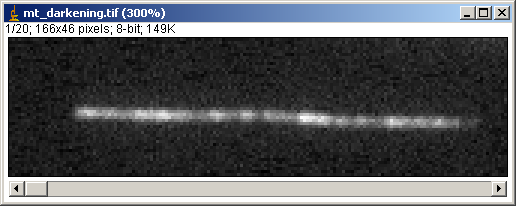
\includegraphics[scale=0.6]{fig/fig23441_mtStack.png}
\caption{A stack with darkening microtubule}
\label{fig:MTstack}
\end{center}
\end{figure} 

Go back to the first frame and do \ijmenu{[Image -> Adjust -> Thresholding\ldots]}. The image is then automatically adjusted with threshold level. and it seems Ok that the structure is well segmented. But the problem appears as you slid the bar at the bottom. Since image is darkening, area where highlighted decreases. 

%figure
\begin{figure}[htbp]
 \centering
 \subfloat[]{\label{fig:frame1Th}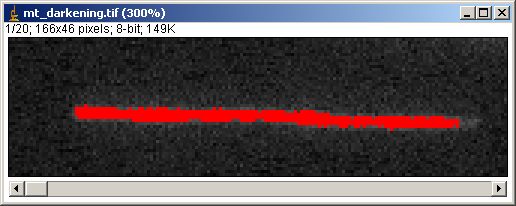
\includegraphics[height = 20mm]{fig/fig23442a_frame1threshold.png}}
 \subfloat[]{\label{fig:framelastTh}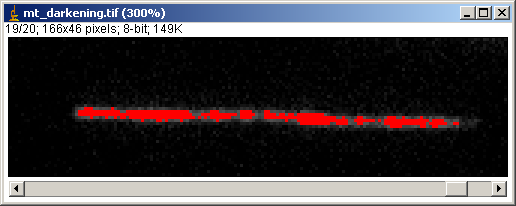
\includegraphics[height = 20mm]{fig/fig23442b_frameLastthreshold.png}}
 \caption{Adjusted with threshold level first frame (a) and the last frame (b)}
 \label{fig:degradingThreshold}
\end{figure}

This is because the threshold minimum and the maximum is kept constant while the intensity of the image is decreasing. To segment the structure while the image darkening is occurring, we must adjust the threshold intensity range as the frame progresses. 
 
The macro below finds the minimum value for the thresholding, that the highlighted area in each frame in a stack is approximately similar to the first frame. \ilcom{while} is used to loop the adjustment until the highlighted area is constant.  Then the threshold is applied to the image to convert the stack to a binary stack. 

\lstinputlisting[morekeywords={*, getThreshold, getSliceNumber, getImageID, getResult, while, setThreshold}]{code/code14.ijm}

%figure
\begin{figure}[htbp]
 \centering
 \subfloat[]{\label{fig:binMTorg}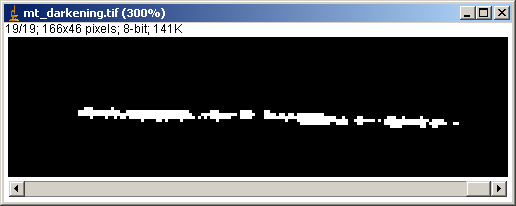
\includegraphics[height = 20mm]{fig/fig23443a_framelastbinOrg.png}}
 \subfloat[]{\label{fig:binMTproc}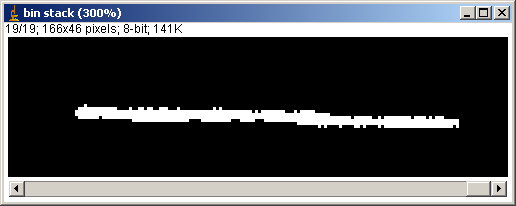
\includegraphics[height = 20mm]{fig/fig23443b_framelastbinProc.png}}
 \caption{Binarized last frame without threshold adjustment (a) and with adjustment using macro (b).}
 \label{fig:ThresholdAdjustResults}
\end{figure}

\begin{itemize}
\item Lines 3 to 5 Check if the active window is a stack. If \ilcom{nSlices==1} (meaning that the image is not a stack), macro is terminated. 

\item Lines 6 to 9: Get the threshold parameter from image and check if the image is adjusted with threshold level. If not, both upper and lower values are -1. In this case, macro is terminated. 

\item Lines 10 to 14: Get stack information. \ilcom{getSliceNumber()} returns the current frame in the stack. Adjusted with threshold level area in this frame (first frame) will be used as the reference area. \ilcom{getImageID()} returns a number that specifically identifies the active window. This ImageID will be used later,by \ilcom{selectImageID(ImageID)} to re-activate the window. 
%\end{itemize}

\begin{indentCom}
\textbf{getImageID()}\\
Returns the unique ID (a negative number) of the active image. Use the selectImage(id), isOpen(id) and isActive(id) functions to activate an image or to determine if it is open or active. 
\end{indentCom}
%\begin{itemize}
\item Line 16: clears the results table without saving. 

\item Line 17: sets the measurement parameter Area, and limits the measurement to the adjusted with threshold level region. 

\item Line 18: Do the measurements. Result is recorded in the first row of the Results table.

\item Line 19: The measured area is stored in the variable ref\_area. 

\item Line 20: temp\_area will be used later in the while loop. 

\item Line 21: the variable ilcom{tol} is a tolerance ratio of error against the reference area. So the adjusted with threshold level area in each frame should be between 97 and 103\% of the reference area. 

\item Line 22: Create a destination stack, where adjusted with threshold level images will be pasted. 

\item Line 23: get the Image ID of newly created image. 

\item Line 25: Loop for the frames starts. 

\item Lines 26, 7: Select the original stack and sets the frame number according to the loop number. \ilcom{selectImageID} works with \ilcom{getImageID} function in line 14. 


\begin{indentCom}
\textbf{selectImage(id)}\\
Activates the image with the specified ID (a negative number). If id is greater than zero, activates the idth image listed in the Window menu. With ImageJ 1.33n and later, id can be an image title (a string).
\end{indentCom}

\item Line 28: Copy the full frame.

\item Lines 29, 30: creates a temporally single frame image and the image copied in line 28 is pasted. 

\item Lines 31 to 37: While loop. temp\_area is evaluated if the area is outside 97 and 103\% of the reference area. If true, then loop continues. Initial temp\_area value is 0 so the loop is at least one time. Set Threshold with lower and upper (line 32). Measure the adjusted with threshold level area, and then lower is incremented -1. The area is evaluated, and if it does not meet the criteria set in line 31, then the loop continues with wider threshold range. 

\item Lines 38 to 40: The adjusted with threshold level image will be converted to black \& white image and then copied. The single frame temporary image is closed.

\item Line 41, 42: destination stack is activated and the same frame as the source stack is set. 

\item Line 43: Binarized image in the clipboard is pasted into the destination stack.

\item Line 44: returns to Line 25 until all stack frames are processed.

\item Line 45: Terminates the macro. 
\end{itemize}

